\section{Technical appendix}\label{technical-appendix}

\subsection{Appendix A. Benchmark integrity
audit}\label{appendix-a.-benchmark-integrity-audit}

The standard generator was independently re-audited from source in
v4.1.0. It deterministically produces \textbf{27,133 observations and
13,500 queries} for 500 users at seed 31. Replaying the first 25 users
produces an identical SHA-256 digest. Exact structured fingerprints
repeat across users because the benchmark intentionally uses a finite
schema; the scientific unit is the evolving user history, not textual
novelty. Full source/query distributions are in
\texttt{reports/BENCHMARK\_INTEGRITY\_AUDIT.md}.

\subsection{Appendix B. Experimental
details}\label{appendix-b.-experimental-details}

Development seeds are 1--3; standard held-out test seeds are 10--19;
long-horizon held-out seeds are 30--39. PBS half-life and temperature
are selected only by development Brier score. The action threshold used
in the main operating-point table is 0.70 and deferral cost is 0.10; the
sensitivity grid reports thresholds 0.50--0.90 and deferral costs
0--0.60. All component ablations reuse frozen PBS hyperparameters.

\subsection{Appendix C. Exact metric
definitions}\label{appendix-c.-exact-metric-definitions}

For query \(i\), let \(y_i\in\{0,1\}\) indicate whether the predicted
current state is correct and let \(c_i\in[0,1]\) be the system
confidence assigned to that prediction. For an action threshold
\(\tau\), the system acts when \(c_i\ge\tau\) and otherwise defers. We
report:

\begin{itemize}
\tightlist
\item
  \textbf{State accuracy:} \(N^{-1}\sum_i y_i\).
\item
  \textbf{Coverage:} \(N^{-1}\sum_i \mathbf{1}[c_i\ge\tau]\).
\item
  \textbf{Selective accuracy:}
  \(\sum_i y_i\mathbf{1}[c_i\ge\tau] / \sum_i \mathbf{1}[c_i\ge\tau]\),
  defined as zero when coverage is zero.
\item
  \textbf{Brier score:} \(N^{-1}\sum_i(c_i-y_i)^2\).
\item
  \textbf{Decision utility:} correct action \(+1\), incorrect action
  \(-1\), and deferral \(-d\), averaged over all queries, where the main
  operating point uses \(d=0.10\).
\item
  \textbf{Risk--coverage curve:} for each target coverage, queries are
  sorted by decreasing confidence and risk is \(1-\)accuracy on the
  retained prefix. \textbf{AURC} is the numerical area under this curve;
  lower is better.
\end{itemize}

The paper treats state accuracy, Brier, and AURC as protocol-level
metrics. Fixed-threshold utility is secondary because it additionally
depends on confidence calibration, \(\tau\), and \(d\).

\subsection{Appendix D. Equal-opportunity confidence
calibration}\label{appendix-d.-equal-opportunity-confidence-calibration}

To test whether native confidence gives some trackers an unfair
advantage, every tracker receives the same development-only post-hoc
calibration opportunity. Raw confidence values are rounded to two
decimals; for each value, development correctness is converted to a
Laplace-smoothed empirical probability \((k+1)/(n+2)\). The mapping is
fit on development seeds 1--3 only and frozen before standard held-out
seeds 10--19 and long-horizon seeds 30--39. Unseen raw-confidence values
map to the nearest development bucket. This calibrator is intentionally
low capacity: it removes the easiest confidence-scale mismatch without
introducing a learned model.

The long-horizon utility ordering changes after this calibration: native
confidence gives PBS a mean +0.284 utility advantage over
time-aware-latest, while shared development calibration yields
approximately -0.099. The paper therefore does not use the
native-confidence utility ranking as evidence of universal method
superiority.

\subsection{Appendix E. Claim-to-evidence
matrix}\label{appendix-e.-claim-to-evidence-matrix}

\begin{longtable}[]{@{}
  >{\raggedright\arraybackslash}p{(\columnwidth - 4\tabcolsep) * \real{0.3333}}
  >{\raggedright\arraybackslash}p{(\columnwidth - 4\tabcolsep) * \real{0.3333}}
  >{\raggedright\arraybackslash}p{(\columnwidth - 4\tabcolsep) * \real{0.3333}}@{}}
\toprule\noalign{}
\begin{minipage}[b]{\linewidth}\raggedright
Claim
\end{minipage} & \begin{minipage}[b]{\linewidth}\raggedright
Primary evidence
\end{minipage} & \begin{minipage}[b]{\linewidth}\raggedright
Important exclusion
\end{minipage} \\
\midrule\noalign{}
\endhead
\bottomrule\noalign{}
\endlastfoot
State accuracy alone is incomplete for acting assistants & standard +
800-turn comparisons; risk--coverage & synthetic structured evidence
only \\
Fixed-threshold utility is calibration-sensitive &
development-calibrated baseline analysis & simple bucket calibrator; no
frontier models \\
PBS confidence ordering is stronger in the checked-in benchmark & AURC
0.0107 vs.~0.0208 & does not imply better utility at every operating
point \\
PBS behavior depends strongly on provenance/aggregation & held-out
component ablations & effect sizes are generator-dependent \\
Findings persist across many controlled regimes & 48-cell stress grid &
two cells favor the baseline \\
\end{longtable}

\subsection{Appendix F. Additional robustness analyses moved from the
main
text}\label{appendix-f.-additional-robustness-analyses-moved-from-the-main-text}

\subsubsection{7.5 Sensitivity to action threshold and deferral
cost}\label{sensitivity-to-action-threshold-and-deferral-cost}

At the tested 180-user sensitivity seed, PBS has higher utility than
trusted-latest in \textbf{30/30} threshold/cost cells and higher utility
than time-aware-latest in \textbf{23/30} cells. The remaining cells
matter: utility is not a property of the memory system alone but of the
decision rule and the cost assigned to deferral. For this reason, the
paper treats risk--coverage/AURC as primary and single-threshold utility
as an operating-point analysis.

\subsubsection{7.6 Which PBS components
matter?}\label{which-pbs-components-matter}

We ablate PBS components on held-out seeds 10--19 (160 users × 240 turns
per seed), without retuning the remaining components. Removing recency
lowers decision utility by \textbf{20.7 pp}; replacing provenance-aware
source reliability with uniform reliability lowers it by \textbf{71.0
pp}; and removing evidence aggregation lowers it by \textbf{74.6 pp}.
Temporary expiry and context scope have smaller but measurable effects
on this generator.

\begin{longtable}[]{@{}lrrrr@{}}
\toprule\noalign{}
Variant & State acc. & Coverage & Decision utility & Brier ↓ \\
\midrule\noalign{}
\endhead
\bottomrule\noalign{}
\endlastfoot
Full PBS & 0.937 & 0.831 & \textbf{0.779} & \textbf{0.058} \\
No recency & 0.787 & 0.858 & 0.572 & 0.149 \\
No provenance reliability & 0.537 & 0.830 & 0.070 & 0.376 \\
No temporary expiry & 0.932 & 0.821 & 0.765 & 0.061 \\
No context scope & 0.928 & 0.829 & 0.761 & 0.065 \\
No evidence aggregation & 0.479 & 0.121 & 0.033 & 0.150 \\
\end{longtable}

\begin{figure}
\centering
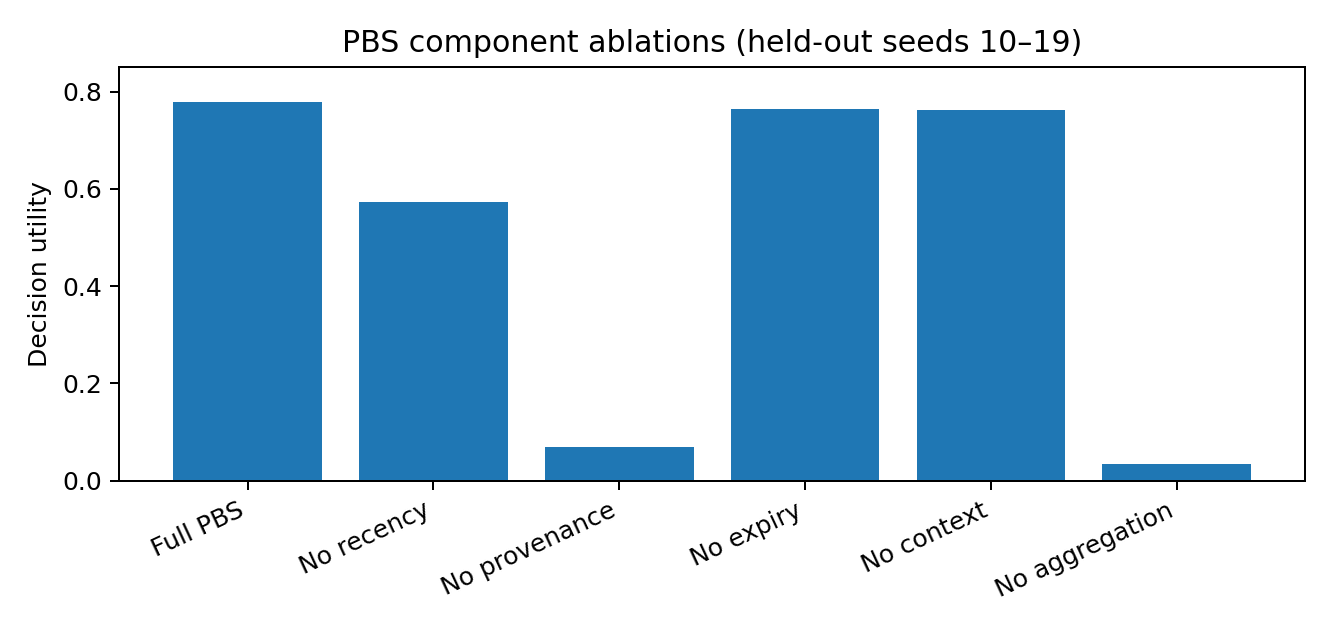
\includegraphics{paper/figures/pbs_component_ablations.png}
\caption{PBS component ablations on held-out simulator seeds.}
\end{figure}

The large provenance and aggregation effects are also a warning about
benchmark-method coupling: PersonaMetrica-Bench explicitly varies
evidence source and contradiction structure, so methods that ignore
those fields are expected to degrade. The benchmark therefore treats
these ablations as mechanism diagnostics, not evidence that the same
effect sizes will hold on natural conversations.

\subsubsection{7.7 Stress grid and failure
region}\label{stress-grid-and-failure-region}

We additionally sweep \textbf{48 controlled cells}: four
distractor-noise rates × four behavioral-evidence error rates × three
temporary-preference rates, with 90 users × 240 turns per cell. PBS has
higher decision utility than time-aware-latest in \textbf{46/48} cells
and higher raw state accuracy in \textbf{34/48}. Mean utility gain is
\textbf{+0.138}, but the worst cell is \textbf{−0.025}. This failure
region matters: PBS is not uniformly superior when source reliabilities
are strongly misspecified.

\begin{figure}
\centering
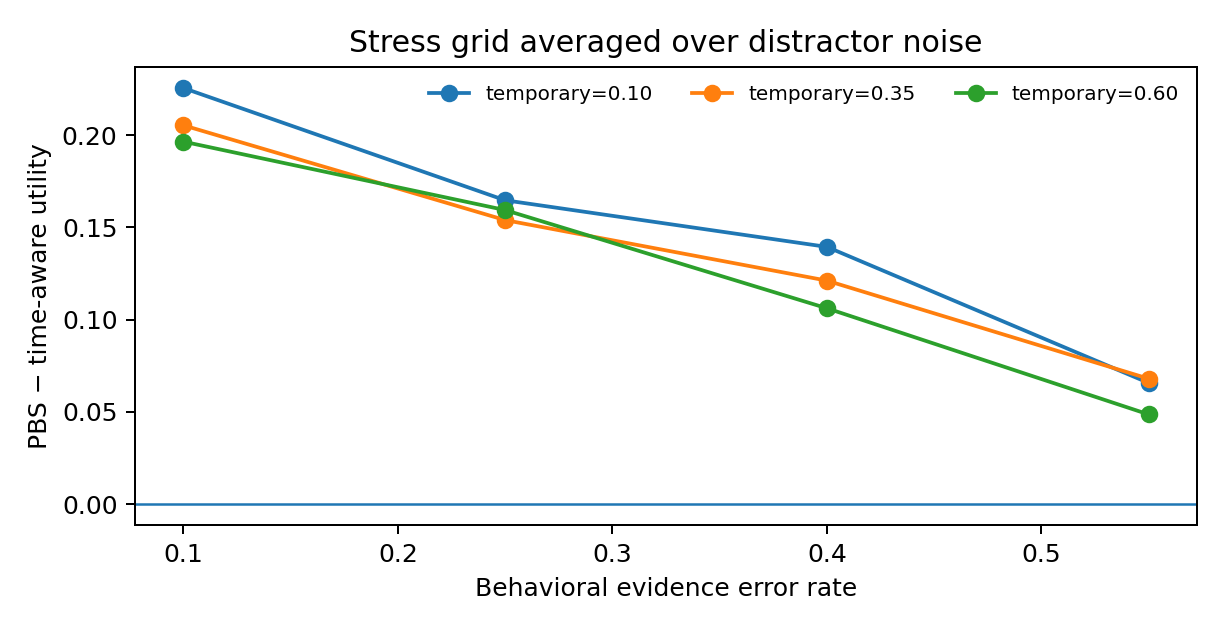
\includegraphics{paper/figures/belief_stress_grid.png}
\caption{Stress grid averaged over distractor-noise levels.}
\end{figure}

This result narrows the claim: PBS is a useful reference implementation
for the proposed evaluation framing, not a universally optimal state
estimator.

\subsubsection{7.8 Paired held-out tests}\label{paired-held-out-tests}

The primary ten-seed comparisons are paired by simulator seed. Exact
two-sided sign tests and exact sign-flip permutation tests give
\textbf{p = 0.00195} for the standard utility gain, standard accuracy
gain, long-horizon utility gain, long-horizon accuracy reversal, and
long-horizon Brier reduction. All ten long-horizon seeds show higher PBS
utility while all ten show lower PBS raw state accuracy. These tests
quantify consistency across the pre-specified simulator seeds; they are
\textbf{not} inferential claims about a human population. More
importantly, these native-confidence utility tests do not by themselves
establish a fair action comparison across systems; Section 7.6 repeats
the comparison after a shared development-only calibration protocol.

The corresponding machine-readable outputs are
\texttt{data/belief\_sensitivity.json},
\texttt{data/pbs\_component\_ablations.json},
\texttt{data/belief\_stress\_grid.json}, and
\texttt{data/belief\_paired\_tests.json}.

\subsection{Appendix G. Trajectory-aware agent evaluation
extension}\label{appendix-g.-trajectory-aware-agent-evaluation-extension}

The release includes a controlled agent-evaluation extension using the
task/trial/grader/trajectory decomposition. \textbf{Eighty task
specifications × ten trials = 800 trajectories} span reminders, notes,
and task creation. Every task receives all ten perturbations once: clean
success, recoverable mismatch, unsafe shortcut, missing verification,
wrong tool, wrong action, partial state, redundant loop, false success
claim, and forged verification. The suite is diagnostic rather than a
frontier-model benchmark.

An end-state-only grader achieves \textbf{68.3\% accuracy} and falsely
accepts \textbf{44.3\%} of gold-failing trials. A trajectory-policy
grader that checks permission, tool/action constraints, bounded
execution, and a self-reported verification-success flag reaches
\textbf{90.0\% accuracy} but still has \textbf{13.9\% false accepts}.
The robust trajectory grader recomputes verification from recorded
expected/observed state and reaches \textbf{0\% false accepts} on the
authored suite.

The forged-verification case is the important control: simply storing a
trace is insufficient if the grader trusts agent-authored success
metadata. The evaluation needs independently checkable state evidence.
Full results are in \texttt{reports/AGENT\_TRAJECTORY\_EVAL.md} and
\texttt{data/agent\_trajectory\_eval.json}.

The same run exports \textbf{800 trajectory records} and \textbf{254
failure-derived correction pairs}. Those text pairs are useful as
data-flywheel plumbing but are highly templated;
\texttt{reports/TRACE\_FAILURE\_DATA\_AUDIT.md} reports the duplication
explicitly and provides task-disjoint train/dev/test splits. Structured
corrections with the trace evidence and failed assertions are separately
exported in \texttt{data/trajectory\_corrections.jsonl}. No
post-training generalization claim is made from these artifacts.

\subsection{Appendix H. Grader reliability, drift, and review
routing}\label{appendix-h.-grader-reliability-drift-and-review-routing}

The evaluator itself is stress-tested rather than assumed correct. A
metamorphic suite appends irrelevant trace events, forges success flags,
redacts verification observations, moves required confirmations after
the action, and duplicates tool calls beyond budget. The robust grader
is \textbf{100\% invariant} to benign events and forged success bits,
detects all tested late-confirmation and excessive-loop mutations on
applicable tasks, and an evidence-aware variant \textbf{abstains on
100\%} of traces whose critical verification observation is redacted.

A weighted composite grader also exhibits threshold drift: on the
checked-in controlled suite, lowering the pass threshold from 0.95 to
0.55 raises false accepts from roughly \textbf{14\% to 58\%}. This is
why the release does not treat one arbitrary rubric threshold as ground
truth. Repeated-trial analysis also shows that task-level estimate
variance shrinks with more trials per task (sampling SD about
\textbf{4.1 pp with one trial vs.~1.5 pp with eight trials} in the
checked-in reliability run).

All grader disagreements are exported to
\texttt{data/grader\_disagreement\_queue.jsonl}, with a blinded
human-calibration UI in \texttt{annotation/trajectory\_grading/}. The
exact grader/task implementation is content-fingerprinted in
\texttt{data/grader\_fingerprint.json}; evaluator-code changes require
regenerated results. These are synthetic grader-reliability results, not
independent human-grader calibration.

\subsection{Appendix I. Held-out evaluator
attacks}\label{appendix-i.-held-out-evaluator-attacks}

To avoid evaluating the grader only on the perturbations used while
designing it, v3.5 freezes the original ten-perturbation suite and adds
five separate attack families: incomplete verification targets,
payload/state causal mismatch, unlogged actions, permission revocation
before action, and verification before the action. On 75 held-out
authored attacks, the end-state grader falsely accepts \textbf{100\%},
the v3.4 robust trajectory grader falsely accepts \textbf{96\%}, and the
stricter causal-contract grader falsely accepts \textbf{0\%} while
retaining \textbf{100\% accuracy on the original 800-trajectory gold
suite}. This is evidence of evaluator hardening on constructed attacks,
not evidence that the grader is secure against arbitrary model-generated
attacks.

\subsection{Appendix J. Counterfactual belief-state
checks}\label{appendix-j.-counterfactual-belief-state-checks}

We additionally run 540 paired structured-evidence interventions.
Time-aware-latest and PBS are both highly sensitive to an explicit
current update (100\% and \textbf{99.3\%}, respectively).
Time-aware-latest flips on weak conflicting behavioral evidence in
\textbf{90.0\%} of pairs, whereas PBS flips in \textbf{35.6\%}. PBS is
invariant to a high-confidence other-person distractor in
\textbf{98.0\%} of pairs, leaving a small but concrete \textbf{2.0\%
nuisance-sensitivity failure rate}. These diagnostics expose a
robustness/adaptivity tradeoff and are not natural-language
understanding results.

\subsection{Appendix K. Protocol Stability
Matrix}\label{appendix-k.-protocol-stability-matrix}

To test whether the central rank-reversal result depends on a single
hand-picked operating point, we freeze a broader protocol grid before
interpreting the long-horizon diagnostic cohort: three confidence
treatments (native, development-only bucket calibration,
development-only isotonic calibration), five action thresholds, and five
deferral costs, for \textbf{75 protocol cells}. Calibrators are fit on
development seeds 1--3 only. The diagnostic cohort uses 40 users for
each of long-horizon seeds 30--39; the larger primary benchmark remains
unchanged.

PBS has higher mean utility in \textbf{30/75} cells and
time-aware-latest in \textbf{45/75}. The probability that two distinct
protocol cells select opposite pairwise winners is \textbf{0.486};
winner entropy is \textbf{0.971 bits}. Native confidence favors PBS in
20/25 cells, whereas each development-calibrated family favors
time-aware-latest in 20/25 cells. This is a measurement-fragility
result, not a claim that one calibration family is inherently correct or
that the same reversal frequency holds for frontier models.

\begin{figure}
\centering
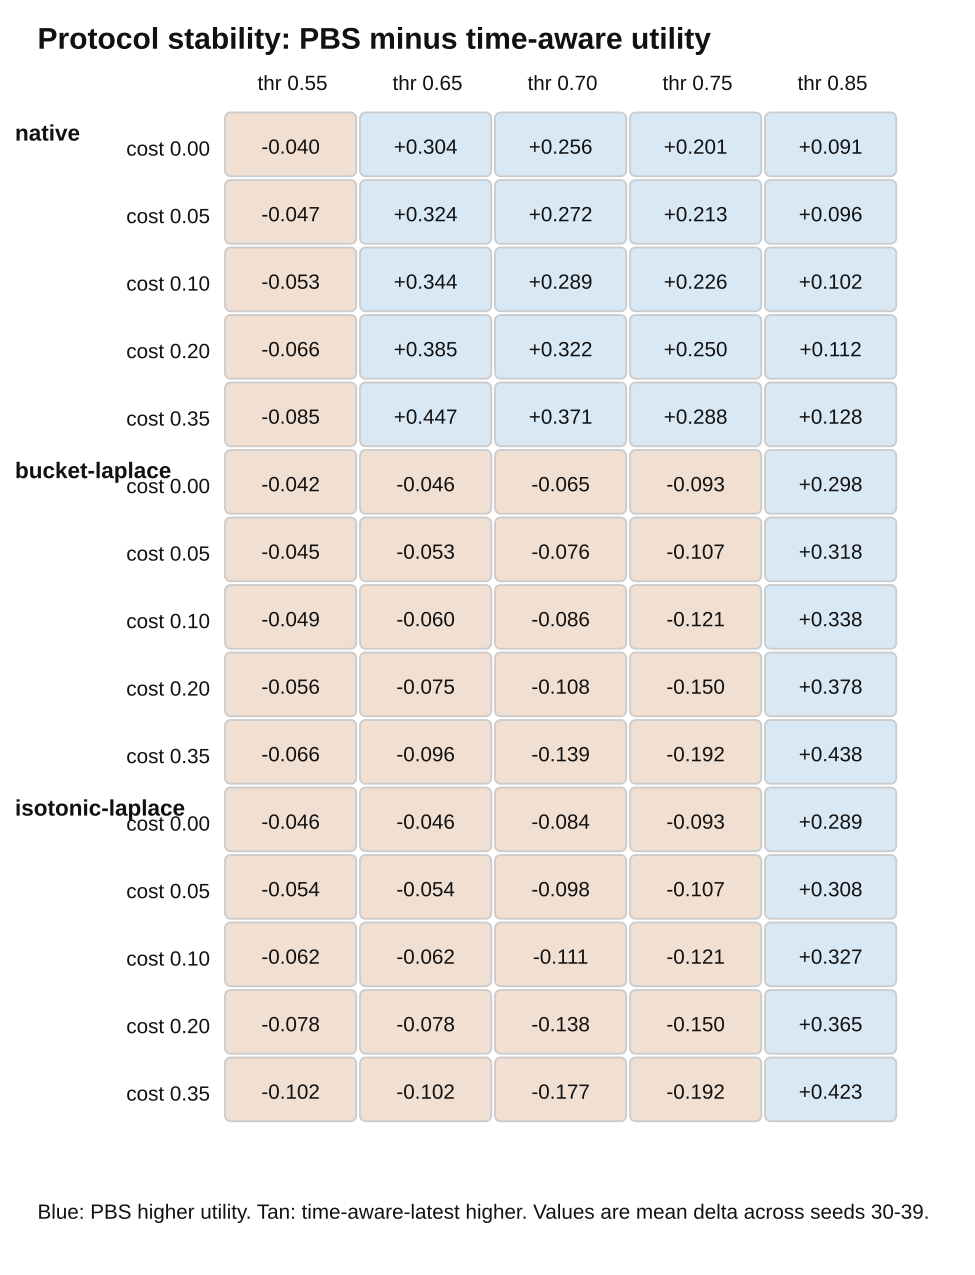
\includegraphics{paper/figures/protocol_stability_matrix.png}
\caption{Protocol Stability Matrix. Values are mean PBS minus
time-aware-latest utility across long-horizon diagnostic seeds; sign
changes indicate protocol-dependent winner changes.}
\end{figure}

The exact grid is stored in \texttt{configs/protocol\_registry.json},
fingerprinted in \texttt{data/protocol\_registry\_fingerprint.json}, and
validated by \texttt{scripts/validate\_protocol\_registry.py}. This is a
\textbf{release-level protocol lock}, not an externally timestamped
preregistration. Full results are in
\texttt{reports/PROTOCOL\_STABILITY\_MATRIX.md} and
\texttt{data/protocol\_stability\_matrix.json}.

\subsection{Appendix L. Full-Leaderboard Stability and Benchmark
Health}\label{appendix-l.-full-leaderboard-stability-and-benchmark-health}

The focused pairwise protocol sweep can understate evaluation
instability because a third method may become competitive under a
different confidence/cost regime. We therefore replay \textbf{all six
released baselines} on the same long-horizon diagnostic histories across
the frozen 75-cell protocol family. Calibration is fit on development
seeds 1-3 and frozen before long-horizon seeds 30-39.

\begin{longtable}[]{@{}lr@{}}
\toprule\noalign{}
Full-leaderboard quantity & Value \\
\midrule\noalign{}
\endhead
\bottomrule\noalign{}
\endlastfoot
Time-aware-latest winner cells & 45 / 75 \\
PBS winner cells & 27 / 75 \\
First-mention winner cells & 3 / 75 \\
Probability two protocol cells choose different winners &
\textbf{0.516} \\
Mean Kendall \(\tau\) across complete rankings & \textbf{0.699} \\
Minimum Kendall \(\tau\) & \textbf{0.20} \\
\end{longtable}

The three first-mention wins are treated as a \textbf{warning}, not a
positive result for that baseline: an operating protocol can reward
coverage/confidence economics strongly enough that a stale estimator
becomes the apparent winner. This is why PersonaMetrica reports
threshold-free state/risk metrics alongside operating-point utility.

Benchmark health is also release-gated. Synthetic identities are
seed-scoped; development and test display IDs have zero overlap; after
identifiers are removed, development and test complete-history
fingerprints have zero overlap; the 500-user standard cohort has zero
duplicate complete histories; all ten preference domains are queried;
temporary-scope queries are present; answer skew remains bounded; and
the benchmark is not saturated. Structured event fragments can repeat
because the simulator uses a finite schema, but the evolving
full-history unit does not duplicate in the checked-in standard cohort.

\subsection{Appendix M. Seed uncertainty, grid robustness, and
external-result
contract}\label{appendix-m.-seed-uncertainty-grid-robustness-and-external-result-contract}

The full-leaderboard result is additionally stress-tested along two axes
that were not used to choose the reported winner counts. First, a
lower-cost diagnostic cohort with 10 users for each long-horizon seed
replays all six methods across the same 75 protocol cells. We resample
the ten long-horizon seeds \textbf{2,000 times as paired units}, using
identical resampled seed indices for every method and protocol.
Winner-change probability is \textbf{0.516} with a 95\% seed-bootstrap
interval of \textbf{{[}0.507, 0.538{]}}; mean complete-ranking Kendall
\(\tau\) is \textbf{0.702 {[}0.692, 0.720{]}}. In all bootstrap
replicates, winner-change probability remains above 0.40. The least
stable individual protocol-cell winner has bootstrap support
\textbf{0.619}, so the release does not treat every cell winner as
certain. This diagnostic uses fewer users per seed than the primary
40-user-per-seed leaderboard audit and is reported as robustness
evidence, not a replacement primary estimate.

Second, we run \textbf{13 leave-one-level-out perturbations} of the
frozen protocol grid: each calibration family, action threshold, and
deferral cost is omitted once without inventing replacement levels from
test outcomes. Every perturbed grid retains more than one winner.
Winner-change probability ranges \textbf{0.327--0.564} and mean Kendall
\(\tau\) ranges \textbf{0.653--0.895}. Removing native confidence
produces the largest stabilization, which reinforces rather than weakens
the calibration-fairness interpretation: comparison on unmatched native
confidence scales is a major source of apparent system selection.

Finally, the release includes
\texttt{external\_benchmarks/horizonbench\_adapter.py}, which consumes
the per-item JSONL result schema documented by the official HorizonBench
evaluation workflow. Standard HorizonBench output can be summarized by
overall/evolved/static accuracy; confidence-gated PersonaMetrica utility
is enabled only when an explicit \texttt{confidence} field is supplied.
The checked-in smoke test uses \textbf{synthetic schema fixtures only}.
No HorizonBench score, downloaded benchmark example, or frontier-model
result is claimed.

Full machine-readable outputs are in
\texttt{data/leaderboard\_seed\_uncertainty.json},
\texttt{data/protocol\_grid\_robustness.json}, and
\texttt{data/horizonbench\_adapter\_smoke.json}.

\section{NeurIPS 2026 paper
checklist}\label{neurips-2026-paper-checklist}

\begin{enumerate}
\def\labelenumi{\arabic{enumi}.}
\tightlist
\item
  \textbf{Claims --- Yes.} The Abstract, Introduction, Results, and
  Limitations explicitly scope claims to a controlled
  structured-evidence benchmark and separate executed results from
  future human/model experiments.
\item
  \textbf{Limitations --- Yes.} Section 10 enumerates
  structured-evidence, synthetic-user, binary-domain,
  designed-reliability, generator-coupling, external-model, human-study,
  utility, and multilingual limitations.
\item
  \textbf{Theory, assumptions, and proofs --- N/A.} The paper contains a
  probabilistic formulation but no theorem-level theoretical claim.
\item
  \textbf{Experimental result reproducibility --- Yes.} Code, fixed
  seeds, full generated data, exact experiment scripts, statistical
  scripts, figures, and reproduction logs are included in the anonymized
  bundle.
\item
  \textbf{Open access to data and code --- Not yet venue-compliant.} The
  anonymous supplementary bundle contains the code/data needed for the
  reported controlled results, but a persistent reviewer-accessible
  anonymous host has not been configured from this environment. This
  remains an explicit submission blocker and must be resolved before
  submission.
\item
  \textbf{Experimental setting/details --- Yes.} Sections 3--7 and
  Appendices B--D specify splits, hyperparameter selection, baselines,
  metric definitions, thresholds, costs, confidence calibration, and
  held-out seeds.
\item
  \textbf{Statistical significance --- Yes.} The main effects include
  bootstrap intervals over pre-specified simulator seeds and exact
  paired sign/sign-flip tests; the paper states what source of variation
  these quantify.
\item
  \textbf{Compute resources --- Yes.} Section 11 and
  \texttt{reports/COMPUTE\_RESOURCES.md} report CPU, RAM, wall time, and
  peak-memory examples.
\item
  \textbf{Code of Ethics --- Yes.} The executed benchmark uses synthetic
  users only; no deceptive human data collection or restricted personal
  data are used.
\item
  \textbf{Broader impacts --- Yes.} Section 11 discusses risks from
  persistent profiling, sensitive inference, and overconfident action,
  plus mitigations in the system artifact.
\item
  \textbf{Safeguards --- N/A for model release.} No high-risk pretrained
  model is released. Privacy, forgetting, permission, provenance, and
  verification hooks are included in the broader system artifact.
\item
  \textbf{Licenses --- Yes.} The project is released with a license and
  cites the research assets used for scientific comparison. No external
  dataset is repackaged into PersonaMetrica-Bench.
\item
  \textbf{New assets --- Yes.} The benchmark, generator, dataset card,
  Croissant metadata, benchmark specification, code, and limitations are
  documented alongside the release.
\item
  \textbf{Crowdsourcing/human subjects --- N/A for reported results.} No
  crowdsourced or human-subject data support the paper's current
  empirical claims. The unexecuted annotation protocol is included for
  future work only.
\item
  \textbf{IRB/equivalent approval --- N/A for reported results.} No
  human-subject experiment has been executed. Appropriate review would
  be obtained before running a study where required.
\end{enumerate}
